\chapter{Borger}

\section{Indledning}
Medicinske teknologier er ikke mulige at anskue uafhængigt af de pågældende individer, der direkte eller indirekte er involveret i teknologien. Disse individer omfatter borgere, patienter, behandlere, forskere, udviklere, politikere og beslutningstagere. Indførelse af en ny medicinsk teknologi kan influere på mange anliggender i forhold til det enkelte individ. I dette afsnit fokuseres på borgeraspektet i forhold til indførelse af virtuel hjemmepleje, og med udgangspunkt i modellen ”Udforskning af patientaspekter i MTV” fra Sundhedsstyrelsens Metodehåndbog for Medicinsk Teknologivurdering berøres følgende aspekter: sociale, kommunikative, økonomiske og individuelle forhold samt etiske aspekter\footnote{Metodehåndbog for Medicinsk Teknologivurdering, side 111}. 
Formålet med afsnittet er at belyse brugen af virtuel hjemmepleje fra et borgerperspektiv. Borgerens oplevelser og erfaringer med brugen af virtuel hjemmepleje ønskes belyst. Desuden ønskes der at give et indblik i, hvilke konkrete borgerbehov levering af virtuel hjemmepleje kan afdække. 
Der gives indledningsvist en introduktion til målgruppen for levering af virtuel hjemmepleje. En klar borgerkarakteristik er nødvendig, idet borgeraspektet afhænger heraf. Definitionen tager udgangspunkt i ’Pilotprojekt Videokommunikation’\footnote{Hvad hedder projektet? I evalueringsreferatet hedder det ’Pilotprojekt Videokommunikation’, mens det i projektplanen kaldes ’Skærmopkald til borgere’} fra Sundhedscenter Hadsten, men er ikke afgrænset hertil. 
Hernæst fremlægges de væsentligste resultater og effekter af virtuel hjemmepleje, og disse inddrages i en analyse af og diskussion om borgernes reaktion på virtuel hjemmepleje. Desuden diskuteres borgernære forudsætninger for en optimalt fungerende virtuel hjemmepleje. Afsnittet afsluttes med en konklusion på resultaterne og dermed en besvarelse på de fokuserede spørgsmål.

\subsection{Fokuserede spørgsmål}
Dette afsnit søger fra et borgerperspektiv at besvare følgende fokuserede spørgsmål: 
Hvilke forudsætninger er der for at video tele conferencing i telesundhed fungerer optimalt?
Spørgsmålet søges besvaret med udgangspunkt i følgende underpunkter:
\begin{itemize}
	\item Brugervenlighed for borgeren
	\item Undervisning af borgeren
	\item Villighed for borgeren
\end{itemize}

Hvordan er brugernes reaktion, og hvad skal man være opmærksom på, opdelt på de sundhedsprofessionelle og borgerne.
Spørgsmålet søges besvaret med udgangspunkt i følgende underpunkter:
\begin{itemize}
	\item something
\end{itemize}	

\section{Litteratursøgning og metode}
\subsection{Litteraturstudie}
Undersøgelsens data og informationer er indhentet gennem litteraturstudier. Videnskabelig litteratur omhandlende videobaserede telesundhedsløsninger for hjemmepleje er søgt på følgende databaser: PubMed, Embase, CINAHL og Cochrane Library. Resultaterne af litteratursøgningsprocessen har været sparsom, idet der ikke forelægger særligt meget videnskabelig evidens på området for virtuel hjemmepleje. På baggrund af implementeringen af virtuel hjemmepleje i Viborg Kommune er der udarbejdet et kandidatspeciale ”Evaluering og dokumentation af telesundhed i kommunal hjemmepleje/sygepleje”. Referencelisten i denne er brugt som inspiration til litteraturstudie og herfra er fundet størstedelen af den videnskabelige litteratur, som anvendes i denne mini-MTV.

\subsection{Generel dataindsamling}
Data er endvidere indhentet gennem møder med forskellige interessenter – Appinux, Netplan Care og medarbejdere i Favrskov Kommune. Møderne har medvirket i afgrænsningen af fokus, og på baggrund af disse møder er problemstillingen konkretiseret yderligere. Der er opnået et afgørende indblik i interessenters interesser i forbindelse med udbredelsen af virtuel hjemmepleje. Desuden er der indhentet viden om, hvorledes en kommune organiserer sig og særligt, hvad kommunal hjemmepleje er karakteriseret ved. På Favrskov Kommunes hjemmeside er der fundet oplysninger vedrørende hjemme- og sygepleje i Favrskov Kommune. Google i al almindelighed er ligeledes benyttet til indhentning af generel information om emnet telesundhed.
 
\subsection{Empirisk dataindsamling }
Empirien i denne mini-MTV er repræsenteret gennem kvalitative metoder i form af strukturerede interviews med deltagere i pilotprojektet i Hadsten Sundhedscenter. Kvalitative metoder søger at give et helhedsbillede af menneskers opfattelse af verden og giver detaljer om mikroprocesser i samfundet. Interviews handler om menneskers subjektive forestilling om dén sociale virkelighed, som de indgår i. Interviews afdækker menneskers viden, opfattelser, meninger og/eller vurderinger om et bestemt emne\footnote{Kilde: Metodehåndbog eller måske noget fra KSS?}. 

\subsubsection{Diskussion af kvalitativ metode}
Med baggrund i de fokuserede spørgsmål har en stor del af fokus været på at belyse borgernes oplevelser og erfaringer med virtuel hjemmepleje. Det har derfor været nærliggende at supplere litteraturstudiet og den generelle dataindsamling med en kvalitativ interviewundersøgelse for netop at opnå en indgående og detaljeret viden om borgernes syn på virtuel hjemmepleje. 

Fra Hadsten Sundhedscenter er der indhentet en kvalitativ evalueringsundersøgelse foretaget blandt deltagere i pilotprojektet. Disse var fem borgere, der modtog virtuel hjemmepleje og to sygeplejersker, der arbejdede med videoopkaldene i den virtuelle hjemmepleje. Evalueringsundersøgelsen var opbygget som et struktureret interview, hvor en sygeplejerske ud fra syv på forhånd definerede spørgsmål interviewede de fem borgere. Disse spørgsmål havde til hensigt at afdække borgerens oplevelser med videoopkald i forhold til konkrete emner og var udformet således, at borgeren skulle svare på et konkret spørgsmål, men mulighed for at tilføje yderligere kommentarer til det pågældende emne. Desuden havde borgeren afslutningsvist mulighed for at supplere evalueringsundersøgelsen med tilføjelser. 

Evalueringsundersøgelsens gyldighed er vurderet med relevans for besvarelsen af de fokuserede spørgsmål. Udarbejdelsen af denne mini-MTV har stor begrænsning i forhold til tid og ressourcer, hvorfor det har været ideelt at medtage evalueringsundersøgelsen fremfor at igangsætte et nyt empirisk vidensgrundlag. Gyldigheden af evalueringsundersøgelsen blev vurderet høj, idet formålet for evalueringsundersøgelsen svarede til denne mini-MTV’s forudsætninger for og krav til empirisk dataindsamling. 

I vurderingen af gyldighed er endvidere medtaget væsentlige overvejelser i forhold til bias. Interviewspørgsmålene er kritisk vurderet for at sikre, at disse har været fyldestgørende i forhold til besvarelsen af de fokuserede spørgsmål i denne mini-MTV. Udvalget af respondenter i interviewundersøgelsen er vurderet tilfredsstillende, idet alle borgere og sygeplejersker med deltagelse i pilotprojektet har deltaget i interviewundersøgelsen. Sammensætningen af respondenterne har dermed ikke været vildledende og har ikke været årsag til bias. Det har ikke været muligt at vurdere bias i forhold til meningspåvirkning af borgeren på et acceptabelt grundlag, da interviewundersøgelsen er foretaget forud for denne mini-MTV. Dog er spørgsmål og svar kritisk diskuteret og analyseret med henblik på at spore eventuelle meningspåvirkninger fra intervieweren – altså sygeplejersken. Idet alle spørgsmål er besvaret, er det vurderet, at der ingen fundamentale misforståelser har været.

Et struktureret interview er karakteriseret ved at teste hypoteser. Et interview med høj struktureringsgrad har god anvendelse, når antallet af respondenter i undersøgelsen er få. Et struktureret interview genererer desuden en overskuelig datamængde sammenlignet med mindre strukturerede interviewundersøgelser. Pilotprojektet, som denne mini-MTV har udgangspunkt i, bestod af en begrænset gruppe borgere, sygeplejersker og øvrige medarbejdere. Formålet med at anvende kvalitativ metode i dette konkrete tilfælde har været at teste hypotesen om, at implementering af virtuel hjemmepleje kan være en medvirkende faktor til at afhjælpe de kommende samfundsmæssige og demografiske udfordringer i Danmark – og i øvrige lande. Med udgangspunkt i disse to omstændigheder sammenholdt med den tids- og ressourcemæssige begrænsning i denne mini-MTV har designet af evalueringsundersøgelsen fra pilotprojektet været passende. 

Motivationen for at vælge kvalitative interviews frem for andre metodedesigns tager afsæt i ønsket om at opnå adgang til respondenternes bevæggrunde, handlemønstre, følelsesliv og erfaringer, hvad angår virtuel hjemmepleje. Ved at sammenholde den empiriske dataindsamling med relevant videnskabelig litteratur er det muligt at opnå en dybere forståelse for borgerens perspektiv. En vigtig essens at pointere ved anvendelsen af de kvalitative interviews er, at disse ikke efterlader mulighed for generalisering.

\section{Målgruppe}
Målgruppen er borgere i ældregruppen\footnote{Ifølge projektplan Skærmopkald til borgere} visiteret til hjemmehjælp karakteriseret ved, at hjemmehjælpen i realiteten ikke kræver fysisk tilstedeværelse af en medarbejder. Målgruppen er altså ældre borgere, der modtager hjælp til at udføre opgaver, som disse med rette påmindelse og støtte selv kan udføre. En klar og entydig aldersmæssig afgrænsning af begrebet ”ældre” synes svær at finde. Denne mini-MTV læner sig op ad Statens Institut for Folkesundhed og afgrænser dermed ”ældre” til at omfatte borgere på 60 år eller derover\footnote{Statens Institut for Folkesundhed, Folkesundhedsrapporten, Danmark 2007 \url{http://www.si-folkesundhed.dk/upload/kap_31_\%C3\%A6ldre_9-5-08.pdf}
}. 

Visitationen af hjemmehjælp med henblik på følgende ydelser: Medicingivning (V og PP), Psykisk pleje og støtte, Vejledning/Rådgivning til struktur i hverdagen, Sundhedspædagogisk indsats, Misbrugsindsats, Sundhedsfremme og forebyggelse, Medicinadministration, Inhalationer, Ernæringsindsats, Indsatser ift. søvn og hvile, Palliation, Psykiatrisk Sygepleje samt Mellemmåltider. Desuden er borgere med mange daglige besøg vurderet med henblik på at kunne isolere enkelte af disse ydelser og levere disse som videoopkald. Af borgere med tilbud om ovenstående ydelser er kun inkluderet de, der er i stand til at betjene en tablet\footnote{Fra evalueringsmøde}.

\section{Resultater}
Som nævnt indledningsvist har afsnittet sit fundamentale udgangspunkt i følgende model, figur(?):

\begin{figure}[H]
	\centering
	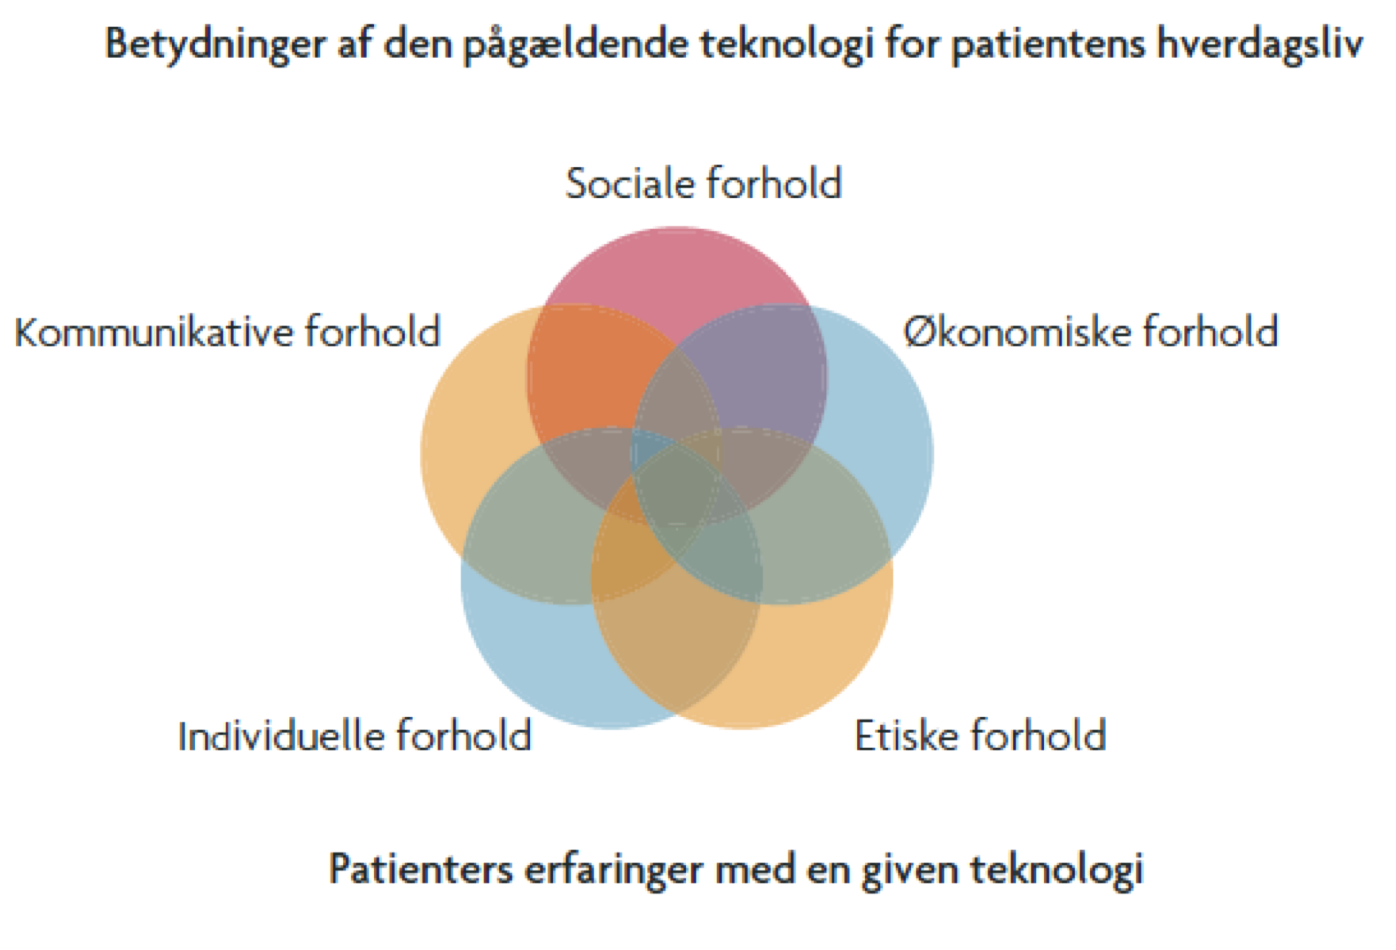
\includegraphics[width=1\textwidth]{Figurer/Snip20160504_25}
	\caption{Udforskning af patientaspektet i MTV \protect\footnotemark}
\end{figure}
\footnotetext{Metodehåndbog for Medicinsk Teknologivurdering, side 111}

Af figuren fremgår det, at de forskellige forhold har en indbyrdes relation, og at disse forhold dermed ikke må eller kan isoleres. Ændringer i ét forhold har indflydelse på de øvrige forhold i en borgers hverdagsliv. Et borgerperspektiv skal dermed anskues ud fra alle disse aspekter, omend nogle har større eller mindre relevans i forhold til en given medicinsk teknologi.

I dette afsnit fremlægges de resultater i forbindelse med virtuel hjemmepleje, som relaterer sig til disse forhold. 

\subsection{Sociale forhold}
Sociale forhold relaterer sig til de sociale betydninger, en given medicinsk teknologi får for borgerens hverdagsliv. Herunder betydninger for borgerens arbejdsliv, familieliv, fritidsliv og livskvalitet. 

Overordnet tyder resultater på, at borgere finder virtuel hjemmepleje meget tilfredsstillende\footnote{Kilde: Videophone delivery of medication management in community nursing}. Ifølge det systematiske review “Virtual Visits in Home Health Care for Older Adults” er tilfredsheden med kvaliteten i hjemmeplejen højere blandt borgere, der modtog virtuel hjemmepleje sammenlignet med borgere, der modtog traditionel fysisk hjemmepleje\footnote{Kilde: Virtual Visits in Home Health Care for Older Adults}. 

For erhvervsaktive borgere betyder virtuel hjemmepleje en større fleksibilitet, da disse borgere ikke er afhængige af et fysisk hjemmeplejebesøg, idet ydelserne kan leveres via videoopkald. Ydelserne kan dermed aftales uden for borgerens normale arbejdstid\footnote{Kilde: Videophone delivery of medication management in community nursing}. 


\section{Kommunikative forhold}
Resultater vedrørende udveksling af information ved brug af videoopkald i virtuel hjemmepleje viser, at videoopkald skaber en koncentreret kommunikation mellem borger og sygeplejerske. Desuden tyder undersøgelser på en forbedring i relationen mellem borgeren og den sundhedsprofessionelle, idet der opleves en mere personlig kontakt mellem borger og sundhedsprofessionel gennem videoopkald\footnote{Kilde: Virtual Visits in Home Health Care for Older Adults}. 

\subsection{Økonomiske forhold}
Ikke relevant. 

\subsection{Individuelle forhold}
Eksistentielle oplevelser i forbindelse med virtuel hjemmepleje peger overordnet på en stor tilfredshed med videoopkald blandt borgere. Ifølge et systematisk review fra 2014 af Husebø og Storm oplever borgerne en formindskelse i ensomhed, en forbedret psykosocial kontakt, en formindskelse i følelsen af være isoleret, en følelse af tryghed og sikkerhed og skabte en følelse af være ”cared for”\footnote{Kilde: Virtual Visits in Home Health Care for Older Adults}.
 
Resultater fra et pilotprojekt i Viborg gennemført i 2013 med afprøvning af videoopkald som alternativ til traditionel fysisk hjemmeplejebesøg viser, at borgeren oplever en mindre grad af stigmatisering, idet virtuel hjemmepleje muliggør diskretion for borgeren. Borgeren kan i fuld fortrolighed kan modtage konkrete ydelser, uden at hjemmeplejens bil er parkeret uden for borgerens hus\footnote{Kandidatspeciale}.

\subsection{Etiske forhold}

\section{Diskussion}
Udforskning af borgeraspekter
\section{Konklusion}